\begin{figure}
    \centering
    \begin{subfigure}{.49\linewidth}
        \centering
        \vspace{-\baselineskip}
        \begin{tikzpicture}[hypergraph,xscale=.8,yscale=0.8,trim left=0cm,trim right=0cm]
            \node[vertex,label={east:$x_1$}] (x1) at (0, 0) {};
            \node[vertex,label={east:$x_2$}] (x2) at (-1, 1) {};
            \node[vertex,label={east:$x_3$}] (x3) at (-1, -1) {};
            \node[vertex,label={west:$x_4$}] (x4) at (1, -1) {};
            \node[vertex,label={west:$x_5$}] (x5) at (1, 1) {};
        
            \begin{scope}[on background layer]
                
                \newcommand*{\pathri}{($(x2) + (-0.25,0.25)$)
                    to[out=45,in=45] ($(x1) + (0.25,-0.25)$)
                    to[out=-135,in=-135] ($(x2) + (-0.25,0.25)$)}
                    
                \newcommand*{\pathrii}{	($(x1) + (0.25,0.25)$)
                    to[out=135,in=135] ($(x3) + (-0.25,-0.25)$)
                    to[out=-45,in=-45] ($(x1) + (0.25,0.25)$)}
                
                \newcommand*{\pathriii}{($(x1) + (-0.25,0.25)$)
                    to[out=45,in=45] ($(x4) + (0.25,-0.25)$)
                    to[out=-135,in=-135] ($(x1) + (-0.25,0.25)$)}

                \newcommand*{\pathriv}{	($(x5) + (0.25,0.25)$)
                    to[out=135,in=135] ($(x1) + (-0.25,-0.25)$)
                    to[out=-45,in=-45] ($(x5) + (0.25,0.25)$)}
                
                \draw[hyperedge,looseness=1,draw=Red,fill=Red,fill opacity=.1] \pathri;
                \draw[hyperedge,looseness=1,draw=Fuchsia,fill=Fuchsia,fill opacity=.1] \pathrii;
                \draw[hyperedge,looseness=1,draw=NavyBlue,fill=NavyBlue,fill opacity=.1] \pathriii;
                \draw[hyperedge,looseness=1, draw=BurntOrange,fill=BurntOrange,fill opacity=.1] \pathriv;
        
                \node[text=Red] at (-1.75,1) {$R_1$};
                \node[text=Fuchsia] at (-1.75,-1) {$R_2$};
                \node[text=Cyan] at (1.75,-1) {$R_3$};
                \node[text=BurntOrange] at (1.75,1) {$R_4$};
                
            \end{scope}
        \end{tikzpicture}
        \vspace{-0.5\baselineskip}
        \caption{Hypergraph of the query}
        \label{fig:star-hg}
    \end{subfigure}
    \hfill
    \begin{subfigure}{.49\linewidth}
        \small
        \centering
        \hfill
        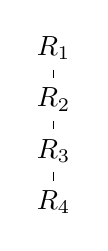
\begin{tikzpicture}[
			level distance=0.65cm,
			level 1/.style={sibling distance=1.2cm},
        ]
			\node { $R_1$ }
				child { node {$R_2$} edge from parent[-]
                    child { node {$R_3$} edge from parent[-]
                        child { node {$R_4$} edge from parent[-] }
                    } 
                };
		\end{tikzpicture}
        \hfill
        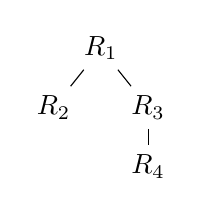
\begin{tikzpicture}[
			level distance=0.75cm,
			level 1/.style={sibling distance=1.2cm},
        ]
			\node { $R_1$ }
				child { node {$R_2$} edge from parent[-]
                }
                child { node {$R_3$} edge from parent[-]
                    child { node {$R_4$} edge from parent[-] }
                } ;
		\end{tikzpicture}
        \hfill
        \ 
        \caption{Two valid join trees}
        \label{fig:star-jts}
    \end{subfigure}
    \vspace{-0.5\baselineskip}
    \caption{Hypergraph and two valid join trees of the star query $Q_{\ref{ex:star}}$ in \cref{ex:star}}
    \label{fig:star}
\end{figure}

